
	\documentclass{article}
	\usepackage{amsmath,amssymb}
	\usepackage{enumitem}
	\usepackage{blindtext}
	\usepackage{booktabs}
	\usepackage{graphicx}
	\usepackage{xcolor}
	\usepackage[vmargin = 1.5in, top = 1in, bottom = 1.2in, letterpaper]{geometry}
	\usepackage{listings}
	\usepackage{courier}
	\lstset{
	basicstyle = \small\tt,
	keywordstyle = \tt\color{blue},
	commentstyle = \it\color[cmyk]{1,0,1,0},
	stringstyle = \tt\color[RGB]{128,0,0},
	%frame = single,
	backgroundcolor = \color[RGB]{245,245,244},
	breaklines,
	extendedchars = false,
	xleftmargin = 2em,
	xrightmargin = 2em,
	aboveskip = 1em,
	tabsize = 4,
	showspaces = false
	}
	\begin{document}
	
	% \newfontfamily\courier{Courier New}

	
	\title{STAT 579 Homework 1}
	\author{Yifan Zhu}
	\maketitle
	
	\begin{enumerate}[leftmargin = 0 em, label = \arabic*., font = \bfseries]
	\item \begin{enumerate}
	\item \begin{lstlisting}[language = R]
> x <- c("group number", "aptitude", "mathematics", "language", "general knowledge")
> score <- read.table(file = "http://maitra.public.iastate.edu/stat579/datasets/student-apt.dat", col.names = x)
	\end{lstlisting}

	\item
\begin{lstlisting}[language = R]
> pairs(score[2:5], col = c("red", "green", "blue")[score$group.number])
\end{lstlisting}
\begin{center}
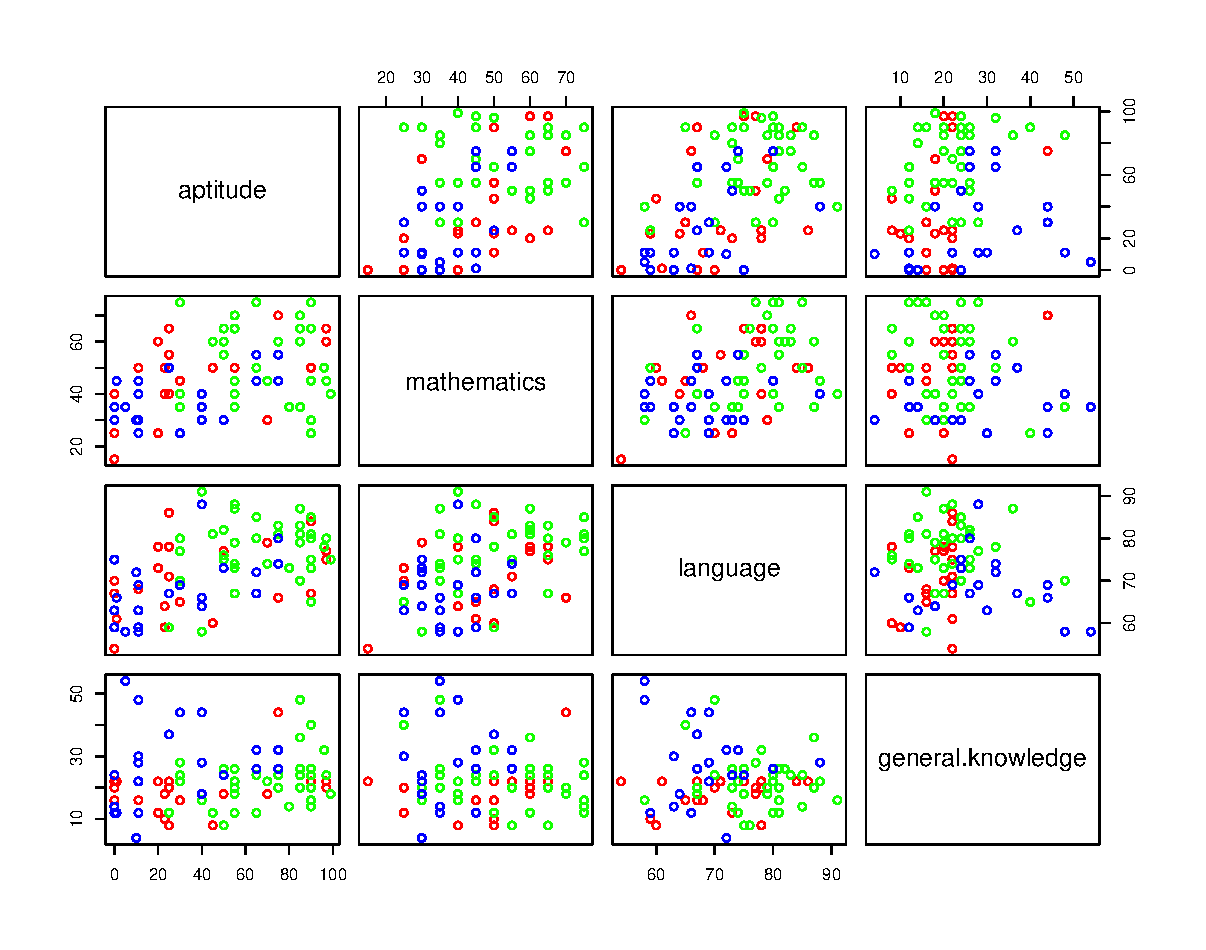
\includegraphics[width = 0.8\textwidth]{Rplot.eps}
\end{center}

\item Comment: It seems that students in Group 1 and 2 have low general knowledge score. Students in Group2 have high apitude and language score. Students in Group 3 have low aptitude score. 
	\end{enumerate}
	
	

	\newpage 

	\item \begin{enumerate}
\item 
\begin{lstlisting}[language = R]
> pidigits <- read.table(file = "http://www.itl.nist.gov/div898/strd/univ/data/PiDigits.dat", skip = 60)
\end{lstlisting}

\item 
\begin{lstlisting}[language = R]
> pifreq <- table(pidigits$V1)
> pifreq <- pifreq[2:10]
> pifreq

  1   2   3   4   5   6   7   8   9 
531 496 461 508 525 513 488 491 521 

\end{lstlisting}

\item 
\begin{lstlisting}[language = R]
> barplot(pifreq)
\end{lstlisting}

\begin{center}
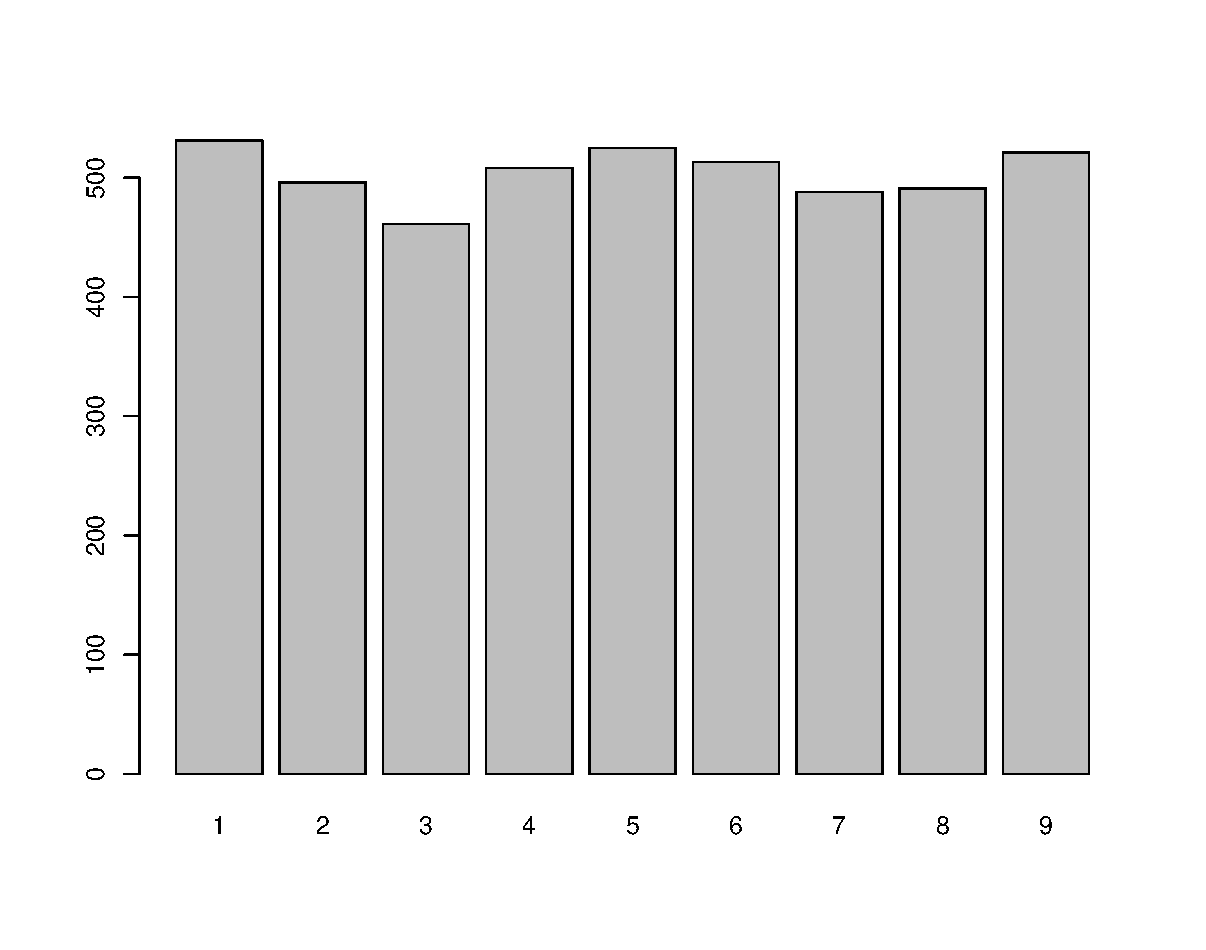
\includegraphics[width = 0.8\textwidth]{barplot.eps}
\end{center}

\item 
\begin{lstlisting}[language = R]
> Xsq <- chisq.test(pifreq)
> Xsq

	Chi-squared test for given probabilities

data:  pifreq
X-squared = 7.7287, df = 8, p-value = 0.4604
\end{lstlisting}

Conclusion: the digits 1 through 9 are equally probable in the digits of $\pi$.
	\end{enumerate}

\newpage
\item 
\begin{lstlisting}[language = R]
> x <- seq(0, 3, 0.01)
> y1 = x^2
> y3 = sqrt(x)
> tobeplot <- data.frame(x = x, y1 = y1, y2 = x, y3 = y3)
> attach(tobeplot)
The following objects are masked _by_ .GlobalEnv:

    x, y1, y3

> rm(x, y1, y3)
> plot(x = x, y = x, "n")
> lines(x = x, y = y1, col = "red")
> lines(x = x, y = y2, col = "green")
> lines(x = x, y = y3, col = "blue")
> abline(v = 1)
> abline(v = 2)
> abline(v = 3)
> detach(tobeplot)
\end{lstlisting}
\begin{center}
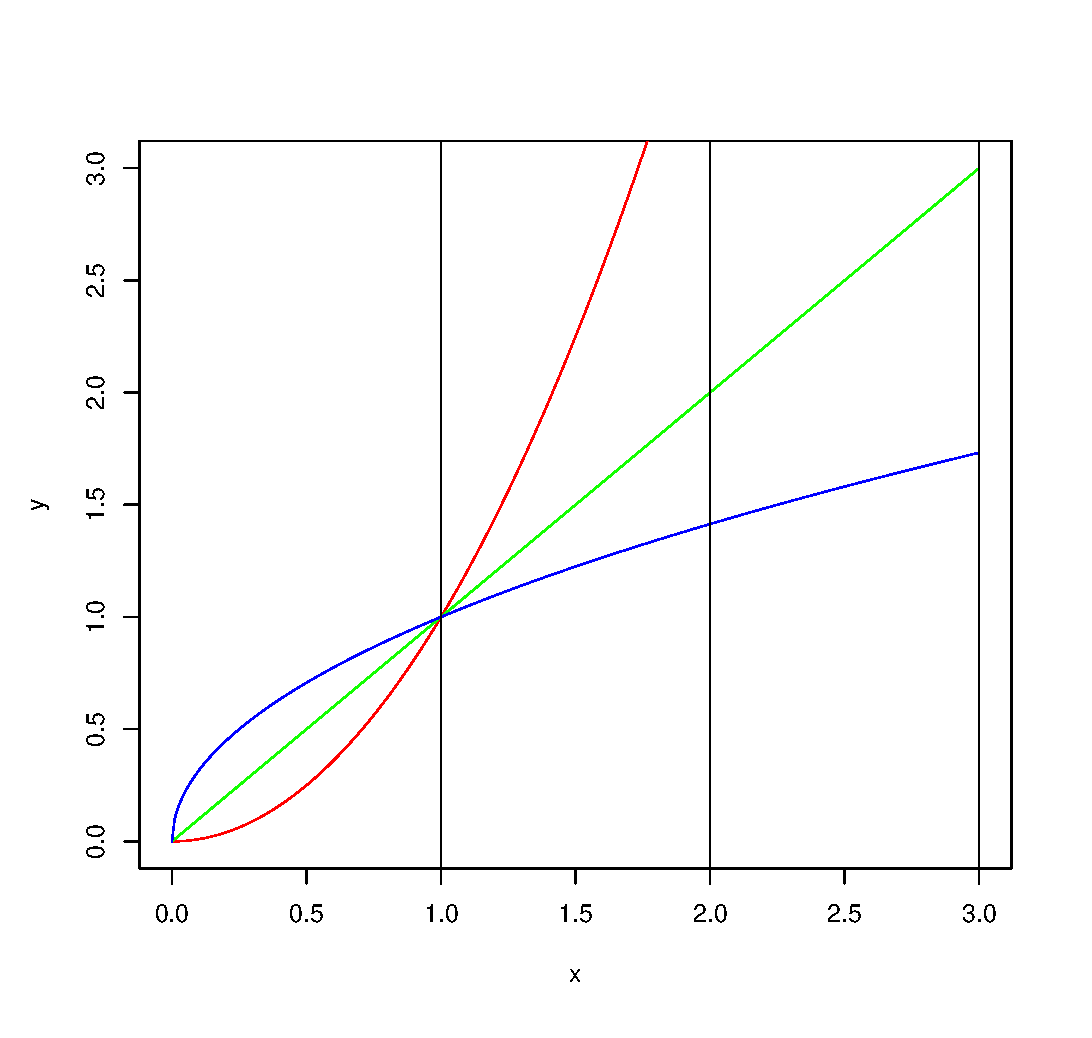
\includegraphics[width = 0.8\textwidth]{plot3.eps}
\end{center}

\newpage
\item \begin{enumerate}
	\item 
\begin{lstlisting}[language = R]
> attach(pressure)
The following object is masked from package:datasets:

    pressure


> temperatureF <- temperature * 9 / 5 + 32
> temperatureF
 [1]  32  68 104 140 176 212 248 284 320 356 392 428 464 500 536 572 608 644 680
 \end{lstlisting}

 \item 
 \begin{lstlisting}[language = R]
> pressureF <- data.frame(temperature = temperatureF, pressure = pressure)
> pressureF
   temperature pressure
1           32   0.0002
2           68   0.0012
3          104   0.0060
4          140   0.0300
5          176   0.0900
6          212   0.2700
7          248   0.7500
8          284   1.8500
9          320   4.2000
10         356   8.8000
11         392  17.3000
12         428  32.1000
13         464  57.0000
14         500  96.0000
15         536 157.0000
16         572 247.0000
17         608 376.0000
18         644 558.0000
19         680 806.0000
\end{lstlisting}

\item 
\begin{lstlisting}[language = R]
> plot(x = pressure, y = temperature, "l", col = "blue")
\end{lstlisting}
\begin{center}
\includegraphics[width = 0.65\textwidth]{pressuretemp.eps}
\end{center}

\item 
\begin{lstlisting}[language = R]
> reg1 <- lm(formula = temperature ~ pressure - 1, data = pressureF)
> summary(reg1)

Call:
lm(formula = temperature ~ pressure - 1, data = pressureF)

Residuals:
   Min     1Q Median     3Q    Max 
-300.2  122.0  247.1  345.2  394.7 

Coefficients:
         Estimate Std. Error t value Pr(>|t|)    
pressure   1.2161     0.2516   4.834 0.000133 ***
---
Signif. codes:  0 ‘***’ 0.001 ‘**’ 0.01 ‘*’ 0.05 ‘.’ 0.1 ‘ ’ 1

Residual standard error: 275.8 on 18 degrees of freedom
Multiple R-squared:  0.5649,	Adjusted R-squared:  0.5408 
F-statistic: 23.37 on 1 and 18 DF,  p-value: 0.000133

> abline(a = 0, b = coef(reg1), col = "red")
\end{lstlisting}
\begin{center}
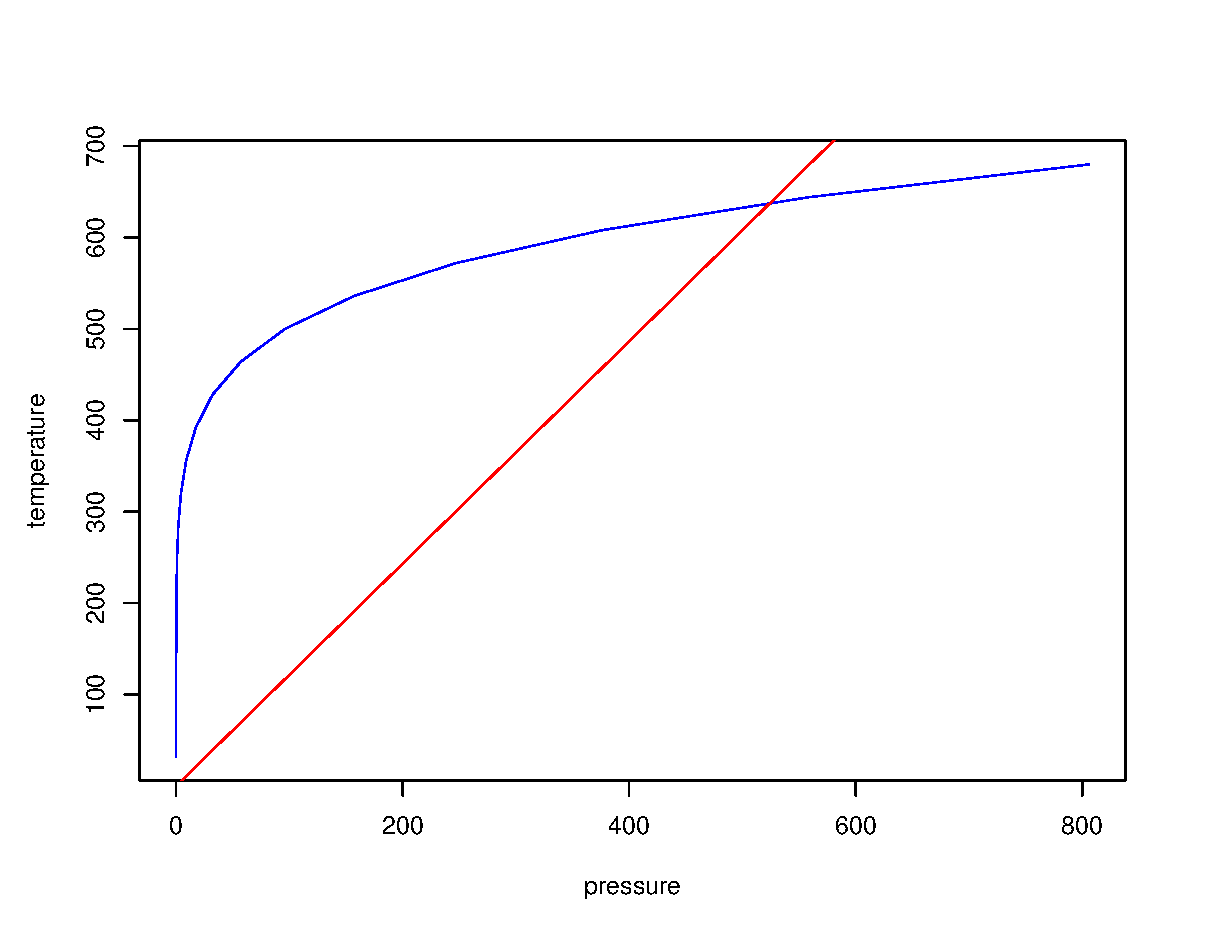
\includegraphics[width = 0.8\textwidth]{reg1.eps}
\end{center}

Comment: According to the summary and the plot, this is not a good model to fit the data. The p-value is small and the fitted result in the plot is not good.


\item 
\begin{lstlisting}[language = R]
> plot(x = fitted(reg1), y = resid(reg1), xlab = "Fitted Values", ylab = "Residuals")
\end{lstlisting}
\begin{center}
\includegraphics[width = 0.8\textwidth]{reg1resid.eps}
\end{center}
Comment: the residuals vary a lot from -300 to 400. some are too big and it seems that they are in a curve rather than randomly distributed around 0.


\item 
\begin{lstlisting}[language = R]
> pressureF2 <- data.frame(temperature = temperatureF, pressure = pressure, pressure2 = pressure^2, pressure3 = pressure^3)
> detach()
> pressureF2
   temperature pressure   pressure2    pressure3
1           32   0.0002 4.00000e-08 8.000000e-12
2           68   0.0012 1.44000e-06 1.728000e-09
3          104   0.0060 3.60000e-05 2.160000e-07
4          140   0.0300 9.00000e-04 2.700000e-05
5          176   0.0900 8.10000e-03 7.290000e-04
6          212   0.2700 7.29000e-02 1.968300e-02
7          248   0.7500 5.62500e-01 4.218750e-01
8          284   1.8500 3.42250e+00 6.331625e+00
9          320   4.2000 1.76400e+01 7.408800e+01
10         356   8.8000 7.74400e+01 6.814720e+02
11         392  17.3000 2.99290e+02 5.177717e+03
12         428  32.1000 1.03041e+03 3.307616e+04
13         464  57.0000 3.24900e+03 1.851930e+05
14         500  96.0000 9.21600e+03 8.847360e+05
15         536 157.0000 2.46490e+04 3.869893e+06
16         572 247.0000 6.10090e+04 1.506922e+07
17         608 376.0000 1.41376e+05 5.315738e+07
18         644 558.0000 3.11364e+05 1.737411e+08
19         680 806.0000 6.49636e+05 5.236066e+08
\end{lstlisting}

\item 
\begin{lstlisting}[language = R]
> attach(pressureF2)
The following object is masked from package:datasets:

    pressure

> reg2 <- lm(formula = temperature ~ pressure + pressure1 + pressure2, data = pressureF2)
Error in eval(expr, envir, enclos) : object 'pressure1' not found
> reg2 <- lm(formula = temperature ~ pressure + pressure2 + pressure3, data = pressureF2)
> summary(reg2)

Call:
lm(formula = temperature ~ pressure + pressure2 + pressure3, 
    data = pressureF2)

Residuals:
    Min      1Q  Median      3Q     Max 
-181.39  -56.54   -2.31   72.88  121.93 

Coefficients:
              Estimate Std. Error t value Pr(>|t|)    
(Intercept)  2.134e+02  2.966e+01   7.195  3.1e-06 ***
pressure     3.417e+00  7.671e-01   4.454 0.000464 ***
pressure2   -8.207e-03  2.826e-03  -2.904 0.010898 *  
pressure3    5.842e-06  2.473e-06   2.362 0.032094 *  
---
Signif. codes:  0 ‘***’ 0.001 ‘**’ 0.01 ‘*’ 0.05 ‘.’ 0.1 ‘ ’ 1

Residual standard error: 98.98 on 15 degrees of freedom
Multiple R-squared:  0.8011,	Adjusted R-squared:  0.7613 
F-statistic: 20.14 on 3 and 15 DF,  p-value: 1.618e-05

\end{lstlisting}
Intercept is significant.

\item 
\begin{lstlisting}[language = R]
> plot(x = pressure, y = temperature, "l", col = "blue")
> lines(x = pressure, y = fitted(reg2), col = "red")
\end{lstlisting}
\begin{center}
\includegraphics[width = 0.7\textwidth]{reg2.eps}
\end{center}
Comment: using this model the fitted result is much better than the previous one according to the plot, but still not good enough.

\item 
\begin{lstlisting}[language = R]
> plot(x = fitted(reg2), y = resid(reg2), xlab = "Fitted Values", ylab = "Residuals")
\end{lstlisting}
\begin{center}
\includegraphics[width = 0.8\textwidth]{reg2resid.eps}
\end{center}
Comment: the varying range of residuals is smaller than the previous one, but it is still large. And they are still like in a curve. 
	\end{enumerate}
 	\end{enumerate}


	
	
	
	\end{document}